\documentclass[11pt]{beamer}
\usepackage[utf8]{inputenc}
\usepackage[T1]{fontenc}
\usepackage{amsmath}
\usepackage{amsfonts}
\usepackage{amssymb}

\usetheme{default}
\usepackage{graphicx}
\begin{document}
    \author{A. Zelenaya \inst{1}, M. Zelenyi \inst{1,2}, A.A.Turinge \inst{1},  V.G. Nedorezov \inst{1}}
    \title{Chemical composition analysis for X-ray transport container scans. }
    %\subtitle{}
    % \logo{}
    \institute[INR]{
        \inst{1} Institute for Nuclear Research RAS \and
        \inst{2} Moscow Institute of Physics and Technology (SU)
    }
    \date{October 10, 2018}
%    \subject{Moscow}
    %\setbeamercovered{transparent}
    %\setbeamertemplate{navigation symbols}{}
    \frame[plain]{\maketitle}
    
    \begin{frame}
        \frametitle{Introduction}
            \begin{columns}
            \begin{column}{0.6\textwidth}
                \begin{itemize}
                    \item For fight against crime, control of transport containers is important.
                    \item For exploring transport containers can be used gamma ray produced by bremsstrahlung
                    \item In this report we consider:
                        \begin{itemize}
                            \item Methodology, existing solution and out proposition.
                            \item GEANT4 simulation of gamma ray scans.
                            \item Measurement resolution of gamma  ray detector
                        \end{itemize}
                   
                \end{itemize}
            \end{column}
            \begin{column}{0.4\textwidth} 
        \includegraphics[width=1\textwidth]{figures/terrorist.jpg}
            \end{column}
        \end{columns}  
    \end{frame}
    \begin{frame}
    \frametitle{Methodology: Gamma ray attenuation}
    \begin{columns}
        \begin{column}{0.7\textwidth}
            $$
            T(E_0, t, Z) = \frac{\int \limits_0^{E_0} S(E_0, E) \exp(-\mu(E,Z)\times t)~dE)}{\int \limits_0^{E_0} S(E_0, E)~dE}
            $$
%            \hline
            \includegraphics[width=1\textwidth]{figures/Attenuation.pdf}
        \end{column}
    \vline~
        \begin{column}{0.4\textwidth} 
            $T$ -  transmittance\\
            $S(E_0, E)$ - response function\\
            $\mu(E,Z)$ - attenuation\\
            $t$ -  optical thickness\\
            $E_0$ -  up-limit energy of bremsstrahlung\\
            $E$ - energy of gamma ray\\
            $Z$ - charge of nuclei 
%            \hline
            \includegraphics[width=1\textwidth]{figures/Bremsstrahlung.pdf}
        \end{column}
    \end{columns}  
\end{frame}

\begin{frame}
    \frametitle{Methodology: Existing solution}
    \begin{block}{Dual energy method}%<1>
        \begin{itemize}
            \item We can't defined Z if optical thickness $t$ is unknown.
            \item But we can use two electron beam with differing energy which give gamma ray with up-limit energy $E^{(1)}_0$ and $E^{(2)}_0$.
            \item Then we can get Z as result of minimizing this function:
            $$
            F(z) = \frac{|t(E^{(1)}_0,z) - t(E^{(2)}_0,z)|}{t(E^{(1)}_0,z)} \to min
            $$
            \item This technique allow to carry scan object to one of four groups: $Z_{eff} \sim 5$, $Z_{eff} \sim 13$, $Z_{eff} \sim 26$, $Z_{eff} \sim 82$.
        \end{itemize}

    \end{block}

\end{frame}

\begin{frame}
    \frametitle{Methodology: Disadvantages and proposition}
    \begin{block}{Disadvantages of dual energy method}%<1>
        \begin{itemize}
            \item It is difficult expose on the target with beams with different energy.
            \item Low efficiency for target which contain elements with strongly differing charges
        \end{itemize}
    \end{block}
    \begin{block}{Our proposition}%<2>
        \begin{itemize}
            \item Use only one electron beam with energy 10 MeV.
            \item Measure not only space distribution, but also energy of gamma ray.
        \end{itemize}
    \end{block}
\end{frame}
%-------------Моделирование 1 часть -------------------
    \begin{frame}
    \frametitle{Simulation: Preliminary estimates}
    \begin{columns}
%        \begin{column}{0.4\textwidth}
%            \begin{itemize}
%                \item 
%                \item 
%                \item 
%                
%            \end{itemize}
%        \end{column}
        \begin{column}{1\textwidth} 
            \includegraphics[width=1\textwidth]{figures/yed_schema_1.pdf}
        \end{column}
    \end{columns}  
\end{frame}

\begin{frame}
    \frametitle{Simulation: Preliminary estimates}
    \begin{columns}
        \begin{column}{0.5\textwidth}
            Very dangerous item\\
            \includegraphics[width=1\textwidth]{figures/Sword.pdf}
        \end{column}
        \begin{column}{0.5\textwidth}
            Uranium cube ( 6cm) in lead sphere (thickness - 1 cm)\\
            \includegraphics[width=1\textwidth]{figures/sim_cube_in_orb.jpeg}
        \end{column}
    \end{columns}  
\end{frame}

\begin{frame}
    \frametitle{Simulation: Preliminary estimates}
    \begin{columns}
        \begin{column}{0.5\textwidth}
            \centering Explosive search\\
            \includegraphics[width=1\textwidth]{figures/sim_hexogen.jpeg}
            
        \end{column}
        \begin{column}{0.5\textwidth}
            Comparison of energy spectrum for aluminium and uranium orb (radius - 1 cm).\\
            \includegraphics[width=1\textwidth]{figures/Difference.pdf}
        \end{column}
    \end{columns}  
\end{frame}

\begin{frame}
    \frametitle{Simulation: Preliminary estimates}
    \begin{columns}
        \begin{column}{0.5\textwidth}
            Energy deposit in detector cells for several material\\
            \includegraphics[width=1\textwidth]{figures/sim_1.jpeg}
            
        \end{column}
        \begin{column}{0.5\textwidth}
            N - number of detector cells
            $$
           \frac{N[E_{dep} < 3~MeV]}
            {N[E_{dep} > 3~MeV]}
            $$
       
            \includegraphics[width=1\textwidth]{figures/sim_2.jpeg}
        \end{column}
    \end{columns}  
\end{frame}
%-------------Моделирование, часть 2 --------------------------
    \begin{frame}
    \frametitle{Simulation: Thickness reconstruction for one dimensional}
    \begin{columns}
        \begin{column}{0.4\textwidth}
            \begin{block}{Simple model}
                Attenuation of gamma ray flux define as:
                                        $$
                \frac{N(E)}{N_0(E)} = \exp(-\sum_i \Sigma^{mean}_i(E)x_i)
                $$
                where $x_i$ --- thickness of $i$-layer, $\Sigma^{mean}_i$ --- mean cross-section for group of material, $N,~N_0$ - number of gamma.
                \begin{itemize}
                    \item Disregard secondary scattering.
                    \item Disregard annihilation line.
                \end{itemize}

                   
            \end{block}

        \end{column}
        \begin{column}{0.55\textwidth}
                  \includegraphics[width=1\textwidth]{figures/yed_schema_2.pdf}
                \begin{block}{Reconstruction algorithm}
                    \begin{itemize}
                        \item Full thickness is known.
                        \item Find thickness using least squares:                  
                        
                    \end{itemize}
                    $$
                    \sum_E(\ln \frac{N(E)}{N_0(E)} + \sum_i \Sigma^{mean}_i(E)x_i))^2 \to min
                    $$
                \end{block}


        \end{column}
    \end{columns}  
\end{frame}
 \begin{frame}
\frametitle{Simulation: Thickness reconstruction for  one dimensional}
\begin{columns}
            \begin{column}{0.4\textwidth}
                \begin{itemize}
                    \item Used Aluminium, Iron and Lead.
                    \item Several sets of thickness with full thickness from 30 cm to 180 cm.
                    \item Energy resolution of detector is 10 \%
                    
                \end{itemize}
            \end{column}
    \begin{column}{0.7\textwidth} 
        \includegraphics[width=1\textwidth]{figures/relError.pdf}
    \end{column}
\end{columns}  
\end{frame}

    \begin{frame}
        %3d -томография
    \frametitle{Simulation: Perspectives}
    \begin{columns}
                \begin{column}{1\textwidth}
                    \begin{itemize}
                        \item If we will use energy-space distribution we can develop algorithm for \textbf{3D-tomography} 
                      
                    \end{itemize}

                \includegraphics[width=1\textwidth]{figures/yed_schema_2.pdf}
                
            \end{column}
    \end{columns}  
\end{frame}

%-------------Экспериментальная часть--------------------------
\begin{frame}
    \frametitle{Experiment: Energy resolution of detector}
    \begin{columns}
        \begin{column}{0.5\textwidth}
            
            \includegraphics[width=1\textwidth]{figures/setup1.png}\\
            Experiment was conduct by Dr. Guber and Dr. Ivashkin.
        \end{column}
                \begin{column}{0.5\textwidth}
            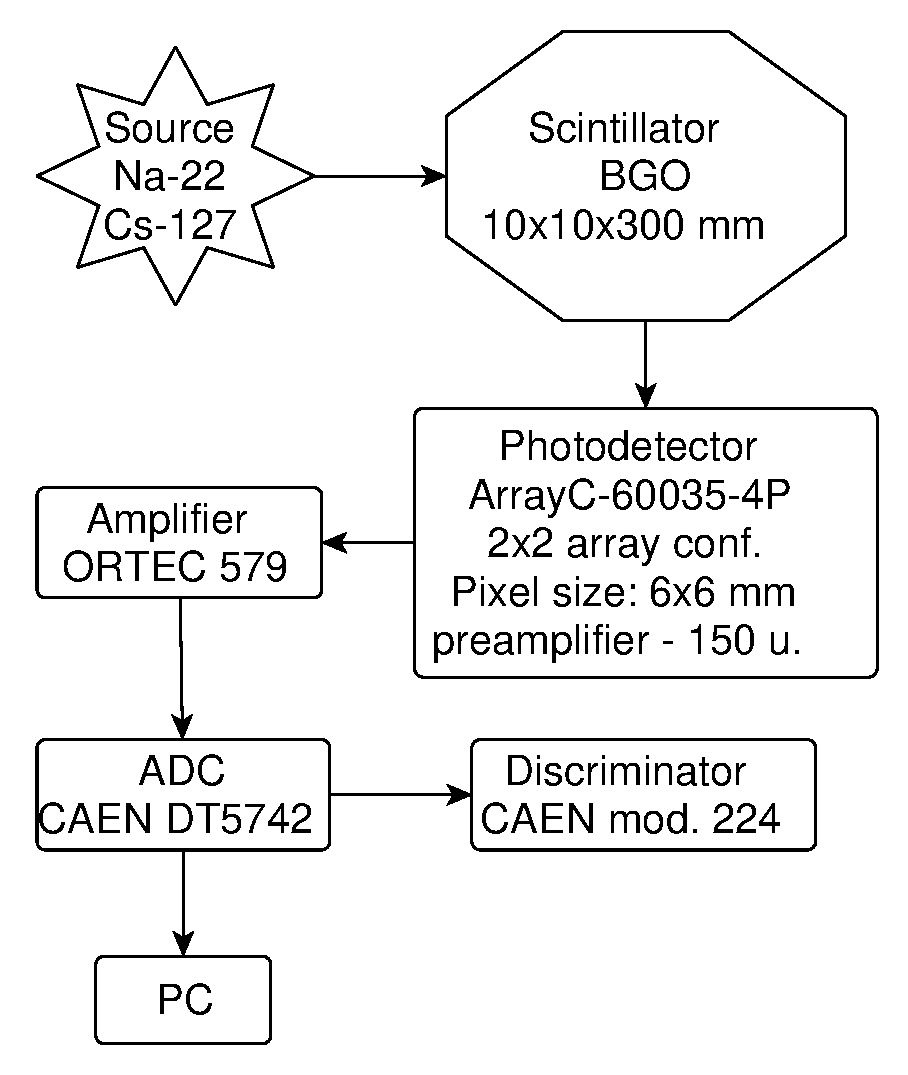
\includegraphics[width=1\textwidth]{figures/yed.pdf}
        \end{column}
    \end{columns}  
\end{frame}

\begin{frame}
    \frametitle{Experiment: Energy resolution of detector}
    \begin{columns}
        \begin{column}{0.5\textwidth}
            $^{22}Na$ --- $0.511~MeV$\\
            \includegraphics[width=1\textwidth]{figures/setup3.png}
            
        \end{column}
                \begin{column}{0.5\textwidth}
                    $^{22}Na$ --- $1.275~MeV$\\
            \includegraphics[width=1\textwidth]{figures/setup4.png}
        \end{column}
    \end{columns} 
    
    \begin{columns}
    \begin{column}{0.5\textwidth}
        $^{137}Cs$ --- $0.662~MeV$\\
        \includegraphics[width=1\textwidth]{figures/setup2.png}
    \end{column}
    \begin{column}{0.5\textwidth}
                Sum of signals from 2 photodiode\\
                Noise threshold: 100 KeV\\
                ~\\
        \begin{tabular}[c]{|c|c|}
             \hline 
            Energy, MeV & Sigma/Mean \\
            \hline 
           0.511 & 14.7\%  \\ 
            \hline 
            0.662 & 19\%\\ 
            \hline 
            1.275 & 13\%\\
            \hline 
        \end{tabular} 
\\

    \end{column}
\end{columns} 
     
\end{frame}

%--------------- Выводы ----------------
\begin{frame}
    \frametitle{Conclusions}
    
    \begin{block}{Results}%<1->   
    \begin{enumerate}
        \item Measurement of gamma ray spectrum allow to identify cargo belonging to group with certain $Z_{eff}$ 
        \item Also its allow to define thickness of layers from different element with accuracy about 25\% 
        \item Studied energy resolution of detector based on BGO scintillator, for photodetector with full array of pixel expected energy resolution about 10\%
    \end{enumerate}
    \end{block}
\begin{block}{Plans and perspectives}%<3->
    With financial support can be developed:
    \begin{enumerate}
        \item Program which check cargo of transport container   for compliance cargo manifest
        \item Algorithm for 3D gamma-tomography.
    \end{enumerate}
\end{block}

\end{frame}

\begin{frame}
    \frametitle{Thank for you attention}
            \includegraphics[width=1\textwidth]{figures/Attenuation.pdf}
\end{frame}

\end{document} 
%
%\begin{frame}
%    \frametitle{}
%\end{frame}
